\documentclass[10pt,a4paper]{article}
\usepackage[margin=1.8cm]{geometry}
\usepackage{fontspec}\setmainfont{Arial}
\usepackage[brazil]{babel}
\usepackage{amsmath,booktabs,graphicx,xcolor,fancyhdr,hyperref,enumitem}
\definecolor{navy}{HTML}{15354D}\definecolor{teal}{HTML}{007F7B}
\hypersetup{colorlinks=true,urlcolor=teal,linkcolor=navy,pdftitle={EJR com termos de troca: replicação preditiva e extensões}}
\pagestyle{fancy}\fancyhf{}\fancyhead[L]{\small EJR com termos de troca}\fancyhead[R]{\small Setembro de 2026}\fancyfoot[C]{\thepage}
\setlength{\headheight}{14pt}\setlength{\parindent}{0pt}\setlength{\parskip}{6pt}
\setlength{\emergencystretch}{3em}
\setlist[itemize]{leftmargin=*,nosep}\renewcommand{\arraystretch}{1.17}
\newcommand{\pagina}[1]{\clearpage{\Large\bfseries\color{navy} #1}\par\vspace{6pt}}
\begin{document}
{\LARGE\bfseries\color{navy} Câmbio nominal de longo prazo:\\EJR com termos de troca}\par
{\large Replicação da equação preditiva e comparação de duas extensões}\par
\textbf{Resultado principal.} Na amostra de seis moedas, acrescentar nível e mudança dos termos de troca não melhora o EJR no agregado. O mesmo ocorre com a cesta de commodities por país. Há ganhos pontuais por moeda, mas eles não se generalizam.

\textbf{Como ler.} A tabela mostra RMSE do modelo dividido pelo RMSE de prever nenhuma mudança no câmbio nominal. Abaixo de 1 melhora a referência. Para justificar a extensão, também é necessário reduzir o erro em relação à coluna EJR. Todas as colunas usam as mesmas observações em cada horizonte.

{\normalsize
\begin{center}\begin{tabular}{lrrr}\toprule
Horizonte & EJR & EJR + termos de troca & EJR + cesta \\ \midrule
1 ano & 1,039 & 1,119 & 1,048 \\
2 anos & 1,076 & 1,229 & 1,086 \\
3 anos & 1,096 & 1,236 & 1,109 \\
4 anos & 1,084 & 1,185 & 1,098 \\
5 anos & 1,037 & 1,092 & 1,060 \\
6 anos & 1,048 & 1,075 & 1,088 \\
7 anos & 1,072 & 1,115 & 1,161 \\
8 anos & 1,115 & 1,188 & 1,247 \\\bottomrule\end{tabular}\end{center}}

\begin{center}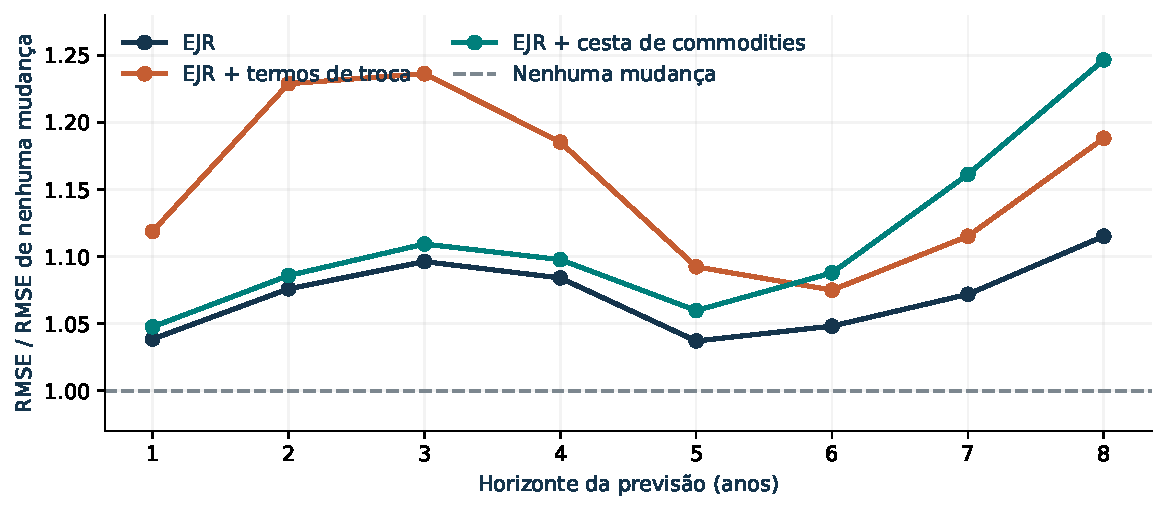
\includegraphics[width=.92\textwidth,height=5.1cm,keepaspectratio]{figures/main.pdf}\end{center}
Em cinco anos, termos de troca elevam o erro agregado em \textbf{5,3\%} frente ao EJR; a cesta o eleva em \textbf{2,2\%}. Brasil e Canadá são exceções pontuais: o primeiro melhora 2,3\% com termos de troca, e o segundo 1,2\% com a cesta.

\textbf{Escopo.} O exercício replica a forma da equação (3.4) de Eichenbaum, Johannsen e Rebelo (2021), aplicada à base atual do projeto. Não reproduz integralmente a amostra histórica, o modelo DSGE ou o bootstrap do artigo. Não há carteiras, decisões de investimento ou alteração dos slides neste estudo.

\pagina{1. O que exatamente foi estimado}
Seja $S_{i,t}$ a cotação em moeda local por dólar e $s_{i,t}=\log S_{i,t}$. Uma variação positiva de $s$ é depreciação da moeda local. O alvo é sempre:
\[y_{i,t,h}=s_{i,t+h}-s_{i,t}.\]
O câmbio real usado como regressor é $q_{i,t}=s_{i,t}+\log P_{US,t-2}-\log P_{i,t-2}$. Defina $\widetilde q^{(t)}_{i,j}=q_{i,j}-\overline q_{i,\leq t}$, com a média calculada exclusivamente até a origem $t$.
\textbf{EJR base, equação (3.4):}
\[y_{i,j,h}=\beta_h\widetilde q^{(t)}_{i,j}+\varepsilon_{i,j,h}.\]
Em cada origem, a inclinação é comum aos países, sem intercepto adicional. A amostra de estimação contém somente origens $j$ cujos alvos já terminaram: $j+h\leq t-1$. A base nova foi conferida contra o código anterior, tanto nos valores previstos quanto nas datas de disponibilidade.

\textbf{Extensão com termos de troca:}
\[y_{i,j,h}=\beta_h\widetilde q^{(t)}_{i,j}+\gamma_h\widetilde z^{(t)}_{i,j}+\delta_h\widetilde{\Delta z}^{(t)}_{i,j}+\varepsilon_{i,j,h}.\]
$z$ é o log dos termos de troca observados. $\Delta z$ é a mudança anual mais recente conhecida na origem. Os regressores adicionais também são centrados pela média de cada país disponível até $t$. O uso de nível permite que uma melhora persistente dos preços relativos altere a previsão; a mudança testa informação adicional da deterioração ou melhora recente.

\textbf{Extensão com cesta de commodities:} a mesma equação, substituindo $z$ pelo índice $c$ da cesta nacional. Nessa extensão, a mudança é $c_t-c_{t-12}$, calculada com preços já disponíveis. Estimamos também cada componente isolado e ambos os conjuntos juntos.

\textbf{Comparação controlada.} Reestimamos todos os coeficientes, inclusive $\beta_h$. Não acrescentamos interceptos, regularização ou métodos diferentes apenas às extensões. Cada painel usa uma máscara comum de dados e as mesmas linhas de treinamento. A especificação conjunta e as variantes isoladas são diagnósticas; as duas comparações principais usam nível e mudança.

\textbf{Relação com o artigo.} O artigo trabalha com dados trimestrais, países e datas ligados aos regimes de metas de inflação. Aqui usamos a base mensal do projeto desde outubro/1999, BRL, EUR, JPY, GBP, CAD e SEK. Os resultados do artigo, portanto, não são uma meta numérica que esta amostra deva reproduzir. O paper encontra ganho agregado acima de dois anos e destaca quatro e seis anos. Testamos explicitamente de um a oito anos, com comparação trimestral adicional. O câmbio real continua sendo um regressor: não estamos prevendo o próprio câmbio real.

\textbf{O que não entra no sinal.} Não usamos os termos de troca efetivamente realizados entre $t$ e $t+h$. A hipótese testada é se informações comerciais já conhecidas ajudam a prever o câmbio nominal futuro.

\pagina{2. Duas medidas que não devem ser confundidas}
\textbf{A. Termos de troca observados, bens e serviços.} Construímos a razão dos deflatores de exportação e importação das contas nacionais:
\[TOT_{i,y}=\frac{X^{corrente}_{i,y}/X^{constante}_{i,y}}{M^{corrente}_{i,y}/M^{constante}_{i,y}}.\]
Os quatro valores vêm do WDI/Banco Mundial, em moeda local. O quociente corrente/constante fornece o deflator implícito. Constantes de base por país desaparecem ao tomar diferenças ou centralizar os logaritmos. Não usamos exportações divididas por importações em valor: isso confundiria preços com quantidades.

O endpoint do índice pronto de bens e serviços não retornou observações. Por isso, a construção usa explicitamente as séries \texttt{NE.EXP.GNFS.CN}, \texttt{NE.EXP.GNFS.KN}, \texttt{NE.IMP.GNFS.CN} e \texttt{NE.IMP.GNFS.KN}. A história precede 1999 para os seis países. Há dados revisados de 2025 para cinco países e de 2024 para o Japão; o calendário do estudo usa no máximo 2024.

\textbf{B. Proxy por cesta nacional de commodities.} Para grupo $k$, sejam $a^X_{ik}$ e $a^M_{ik}$ suas participações nos totais de exportação e importação, médias de 1994--1996. Então:
\[c_{i,t}=\sum_k(a^X_{ik}-a^M_{ik})\,[\log P_{k,t-2}-\log CPI_{US,t-2}].\]
É a contribuição das commodities à razão de duas cestas, supondo que o restante do comércio acompanhe o CPI americano. A cesta usa preços de referência, não os preços efetivos negociados por cada país. Portanto, é uma \textbf{proxy parcial}, não uma medição completa dos termos de troca.

{\normalsize
\begin{center}\begin{tabular}{lrrrr}\toprule
Moeda & Energia & Alimentos & Mat. agrícolas & Metais \\ \midrule
BRL & -12,2\% & 18,3\% & 1,1\% & 6,8\% \\
EUR & -5,8\% & -4,7\% & -1,5\% & -1,2\% \\
JPY & -16,5\% & -16,0\% & -5,6\% & -5,1\% \\
GBP & 2,7\% & -2,7\% & -1,7\% & -0,7\% \\
CAD & 6,0\% & 2,0\% & 7,1\% & 3,2\% \\
SEK & -4,7\% & -4,9\% & 4,1\% & -0,7\% \\\bottomrule\end{tabular}\end{center}}

Pesos negativos identificam maior participação do grupo nas importações. Dentro de cada grupo, a média dos logaritmos dá pesos iguais aos preços: energia (petróleo e gás dos EUA); alimentos (soja, milho e trigo); matérias-primas agrícolas (algodão e borracha); metais (cobre, ferro, alumínio e níquel). A Alemanha aproxima o comércio da área do euro, limitação avaliada retirando EUR.

\textbf{Calendário.} No ano $Y$, termos de troca usam somente $Y-2$ e sua mudança frente a $Y-3$. Não há interpolação. Preços e CPI entram com dois meses de atraso. A sensibilidade usa mais um ano de atraso anual e mais um mês para a cesta. São hipóteses conservadoras de divulgação, não um histórico completo de vintages.

\textbf{Terceira medida, apenas para comparação.} O índice de mercadorias \texttt{TT.PRI.MRCH.XD.WD}, da UNCTAD/WDI, começa em 2005 na extração disponível. Ele é avaliado separadamente. Não emendamos esse índice com a cesta, nem o tratamos como idêntico aos termos de troca de bens e serviços.

\pagina{3. Treinamento e avaliação fora da amostra}
As origens de treino começam em outubro/1999. Cada previsão exige pelo menos 60 origens maduras por moeda, preservando a convenção inicial do código EJR anterior. O teste começa em janeiro/2010 ou na primeira previsão admissível, se posterior. A janela se expande em cada mês; o horizonte muda tanto o fim das origens avaliáveis quanto o início da disponibilidade do modelo.

{\footnotesize
\begin{center}\begin{tabular}{lrrrr}\toprule
Horizonte & Treino no 1º teste & Origens avaliadas & Meses & Meses/h \\ \midrule
1 ano & 1999-10 a 2008-12 & 2010-01 a 2025-08 & 188 & 15,7 \\
2 anos & 1999-10 a 2007-12 & 2010-01 a 2024-08 & 176 & 7,3 \\
3 anos & 1999-10 a 2006-12 & 2010-01 a 2023-08 & 164 & 4,6 \\
4 anos & 1999-10 a 2005-12 & 2010-01 a 2022-08 & 152 & 3,2 \\
5 anos & 1999-10 a 2004-12 & 2010-01 a 2021-08 & 140 & 2,3 \\
6 anos & 1999-10 a 2004-10 & 2010-11 a 2020-08 & 118 & 1,6 \\
7 anos & 1999-10 a 2004-10 & 2011-11 a 2019-08 & 94 & 1,1 \\
8 anos & 1999-10 a 2004-10 & 2012-11 a 2018-08 & 70 & 0,7 \\\bottomrule\end{tabular}\end{center}}

A coluna ``Meses/h'' é apenas uma medida de extensão temporal. Não é uma contagem exata de observações independentes. Seis moedas multiplicam o número de erros, mas não multiplicam a história temporal por seis: choques comuns ligam seus resultados.

\textbf{Exemplo em cinco anos.} Na origem janeiro/2010, o treino contém origens outubro/1999--dezembro/2004, com alvos concluídos até dezembro/2009. A previsão se refere a janeiro/2015. A última origem avaliada é agosto/2021, cujo alvo termina em agosto/2026. Há 140 meses de origem, mas somente 2,3 horizontes de cinco anos em extensão temporal. A informação anual em janeiro/2010 refere-se a 2008 e à mudança 2008/2007.

\textbf{Horizontes comparáveis no mesmo calendário.} Uma checagem adicional restringe todos os horizontes às mesmas 70 origens, novembro/2012--agosto/2018. Essa janela evita atribuir ao prazo diferenças que vêm apenas da seleção de datas. Ela tem ainda menos informação independente nos horizontes longos.

\textbf{Sem sobreposição.} Também avaliamos todas as sequências espaçadas em $h$ meses, variando o mês inicial. Os resultados por offset estão em \texttt{nonoverlap.csv}. Muitas sequências longas contêm somente duas ou três datas; servem como diagnóstico, não como confirmação estatística.

\textbf{Auditoria.} O estudo salva todas as previsões e seus alvos, coeficientes e janelas de treino. Verificações comparam o EJR com a implementação anterior, reproduzem regressões em statsmodels, truncam a base na origem e alteram dados futuros para garantir que a previsão antiga permaneça igual. Outras verificações cobrem defasagens, pesos anteriores à amostra, invariância à base dos índices e preservação dos dados anteriores.

O número anual repetido em doze meses continua sendo \textbf{uma informação anual}. Os 60 meses mínimos de treino não equivalem a 60 observações anuais distintas de termos de troca. A inferência não trata as seis moedas e todos os meses como erros independentes.

\pagina{4. Todas as moedas e todos os horizontes}
RMSE relativo a nenhuma mudança. O agregado reúne os erros quadráticos das seis moedas antes de extrair a raiz; não é a média simples das razões individuais. Valores menores que 1 podem coexistir com piora em relação ao EJR.

\textbf{EJR base}

{\footnotesize
\begin{center}\begin{tabular}{lrrrrrrr}\toprule
Anos & BRL & EUR & JPY & GBP & CAD & SEK & Agregado \\ \midrule
1 & 0,964 & 0,948 & 1,239 & 1,038 & 1,026 & 1,066 & 1,039 \\
2 & 0,916 & 0,917 & 1,344 & 1,178 & 0,991 & 1,194 & 1,076 \\
3 & 0,884 & 0,993 & 1,345 & 1,361 & 0,920 & 1,362 & 1,096 \\
4 & 0,840 & 0,972 & 1,383 & 1,490 & 0,811 & 1,455 & 1,084 \\
5 & 0,792 & 0,899 & 1,379 & 1,537 & 0,709 & 1,434 & 1,037 \\
6 & 0,803 & 0,968 & 1,466 & 1,573 & 0,751 & 1,366 & 1,048 \\
7 & 0,793 & 1,302 & 1,700 & 1,563 & 0,859 & 1,441 & 1,072 \\
8 & 0,816 & 1,226 & 1,869 & 1,445 & 1,161 & 1,482 & 1,115 \\\bottomrule\end{tabular}\end{center}}

\textbf{EJR + termos de troca, nível e mudança}

{\footnotesize
\begin{center}\begin{tabular}{lrrrrrrr}\toprule
Anos & BRL & EUR & JPY & GBP & CAD & SEK & Agregado \\ \midrule
1 & 0,939 & 1,006 & 1,524 & 1,057 & 1,381 & 1,074 & 1,119 \\
2 & 0,886 & 0,956 & 1,803 & 1,167 & 1,520 & 1,204 & 1,229 \\
3 & 0,885 & 0,943 & 1,755 & 1,300 & 1,333 & 1,372 & 1,236 \\
4 & 0,820 & 1,062 & 1,702 & 1,522 & 1,027 & 1,500 & 1,185 \\
5 & 0,774 & 1,014 & 1,523 & 1,653 & 0,838 & 1,505 & 1,092 \\
6 & 0,821 & 1,067 & 1,423 & 1,747 & 0,835 & 1,413 & 1,075 \\
7 & 0,886 & 1,452 & 1,437 & 1,857 & 1,031 & 1,500 & 1,115 \\
8 & 0,947 & 1,456 & 1,517 & 1,901 & 1,462 & 1,598 & 1,188 \\\bottomrule\end{tabular}\end{center}}

\textbf{EJR + cesta de commodities, nível e mudança}

{\footnotesize
\begin{center}\begin{tabular}{lrrrrrrr}\toprule
Anos & BRL & EUR & JPY & GBP & CAD & SEK & Agregado \\ \midrule
1 & 0,967 & 0,946 & 1,284 & 1,038 & 1,012 & 1,068 & 1,048 \\
2 & 0,906 & 0,921 & 1,404 & 1,180 & 0,945 & 1,200 & 1,086 \\
3 & 0,877 & 1,059 & 1,402 & 1,377 & 0,827 & 1,376 & 1,109 \\
4 & 0,848 & 1,015 & 1,413 & 1,498 & 0,767 & 1,476 & 1,098 \\
5 & 0,808 & 0,933 & 1,428 & 1,537 & 0,700 & 1,461 & 1,060 \\
6 & 0,833 & 1,055 & 1,551 & 1,563 & 0,745 & 1,409 & 1,088 \\
7 & 0,855 & 1,516 & 1,923 & 1,563 & 0,839 & 1,529 & 1,161 \\
8 & 0,908 & 1,506 & 2,197 & 1,467 & 1,069 & 1,600 & 1,247 \\\bottomrule\end{tabular}\end{center}}

\textbf{Leitura econômica.} A extensão com termos de troca ajuda modestamente o Brasil em quatro e cinco anos, mas piora o Canadá e outras moedas nesse prazo. A cesta melhora o Canadá em todos os horizontes deste painel, com ganhos pequenos em cinco e seis anos e maiores em três anos. Ainda assim, o Canadá com a cesta perde para nenhuma mudança em um e oito anos. O sinal comercial não funciona da mesma forma em todos os países.

\pagina{5. Onde a informação adicional ajuda}
O mapa mostra a mudança percentual do RMSE contra o EJR. Por exemplo, $-10$ significa redução de aproximadamente 10\% no erro. É uma comparação incremental, distinta de superar nenhuma mudança.
\begin{center}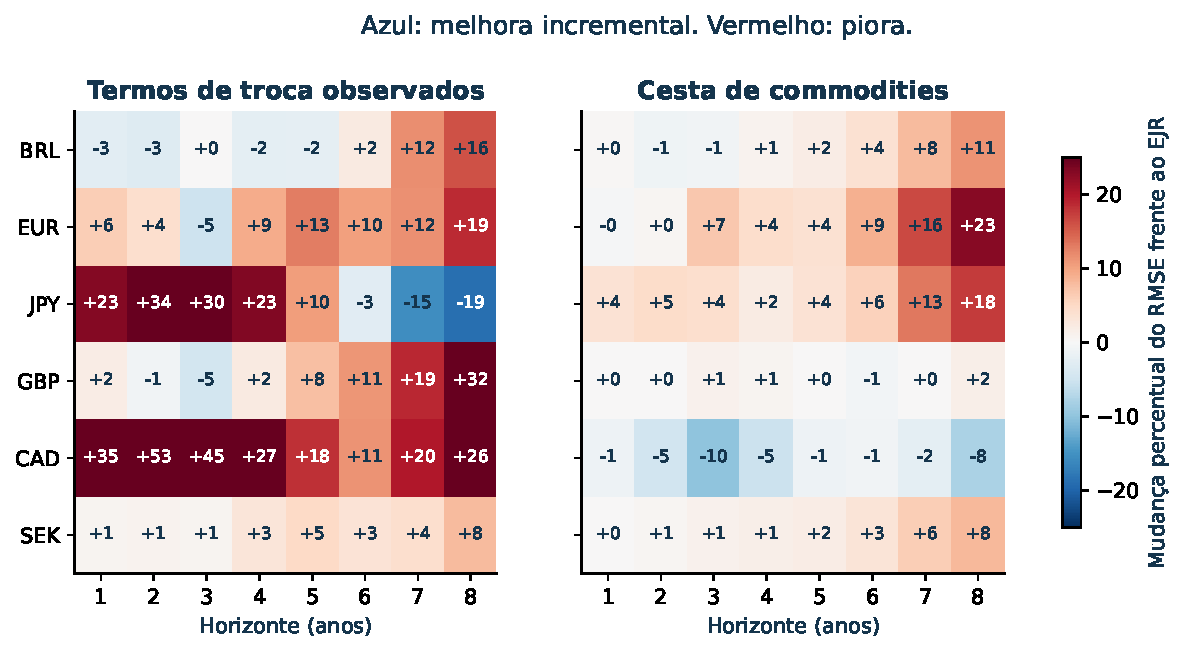
\includegraphics[width=\textwidth]{figures/countries.pdf}\end{center}
\textbf{Cinco anos: Brasil e Canadá.} Termos de troca reduzem o RMSE brasileiro de 0,792 para 0,774 na escala relativa ao passeio aleatório. A cesta reduz o canadense de 0,709 para 0,700. Esses são ganhos descritivos, condicionais à amostra e às demais moedas usadas para estimar as inclinações comuns.
\begin{center}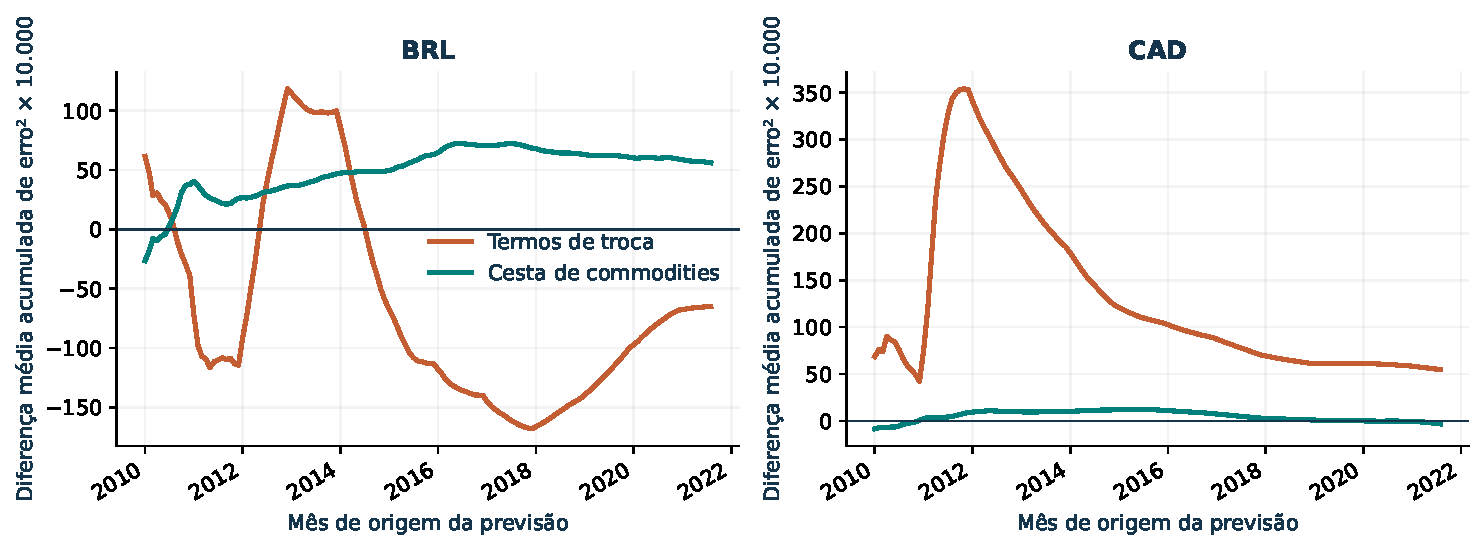
\includegraphics[width=\textwidth]{figures/errors.pdf}\end{center}
O gráfico acumula diferenças de \textbf{erro quadrático de previsão}, não retornos financeiros. Abaixo de zero significa que a extensão acumulou menos erro que o EJR até aquela origem. As previsões são de cinco anos, mesmo quando o eixo horizontal avança mensalmente.

Não selecionamos uma regressão diferente para cada moeda após observar esses resultados. Escolher apenas os países que melhoraram e apresentar a seleção como teste novo criaria outra camada de seleção histórica.

\pagina{6. Robustez e componentes das extensões}
\textbf{Cinco anos, agregado.} Atrasos maiores, observações trimestrais e exclusão de países usam reestimação completa. O numerador e a referência permanecem pareados dentro de cada linha.

{\normalsize
\begin{center}\begin{tabular}{lrrr}\toprule
Variação & EJR & + termos de troca & + cesta \\ \midrule
Principal & 1,037 & 1,092 & 1,060 \\
Maior atraso de divulgação & 1,037 & 1,068 & 1,060 \\
Treino/origens trimestrais & 1,047 & 1,097 & 1,067 \\
Sem BRL & 1,301 & 1,269 & 1,340 \\
Sem EUR & 1,046 & 1,112 & 1,073 \\
Sem BRL e EUR & 1,354 & 1,340 & 1,418 \\\bottomrule\end{tabular}\end{center}}

Sem BRL, termos de troca melhoram em relação ao EJR (1,301 para 1,269), mas ambos perdem para nenhuma mudança. Isso também impede concluir que termos de troca ``nunca ajudam''. O resultado depende da composição do painel. A variante trimestral seleciona fins de trimestre e requer 20 origens maduras; não reconstrói médias trimestrais ou a amostra do artigo.

\textbf{Apenas nível ou apenas mudança.} RMSE relativo ao EJR, agregado. Abaixo de 1 indica ganho incremental. A variante conjunta usa ambos os tipos de informação comercial.

{\footnotesize
\begin{center}\begin{tabular}{lrrrrrrr}\toprule
Anos & TT nível & TT mudança & TT ambos & Cesta nível & Cesta mudança & Cesta ambos & Conjunta \\ \midrule
1 ano & 1,012 & 1,035 & 1,077 & 1,003 & 1,006 & 1,009 & 1,102 \\
2 anos & 1,020 & 1,070 & 1,142 & 1,012 & 1,000 & 1,009 & 1,168 \\
3 anos & 1,026 & 1,059 & 1,128 & 1,011 & 1,002 & 1,012 & 1,129 \\
4 anos & 1,020 & 1,048 & 1,093 & 1,010 & 1,001 & 1,013 & 1,095 \\
5 anos & 1,017 & 1,034 & 1,053 & 1,016 & 1,000 & 1,022 & 1,067 \\
6 anos & 1,017 & 1,020 & 1,026 & 1,034 & 0,993 & 1,038 & 1,021 \\
7 anos & 1,041 & 1,022 & 1,040 & 1,081 & 0,997 & 1,083 & 1,047 \\
8 anos & 1,064 & 1,037 & 1,065 & 1,120 & 0,987 & 1,118 & 1,084 \\\bottomrule\end{tabular}\end{center}}

Isolar a mudança da cesta produz pequenas melhorias contra o EJR em alguns horizontes longos, mas não resolve a comparação com nenhuma mudança. Acrescentar mais regressores pode piorar a estimação: a informação econômica é relevante em princípio, porém a amostra precisa ser suficiente para estimar sua contribuição com estabilidade.

\textbf{Mesmo conjunto de origens em todos os horizontes.} Resultados com nível e mudança, novembro/2012--agosto/2018, relativos ao EJR:

{\footnotesize
\begin{center}\begin{tabular}{lrr}\toprule
Anos & + termos de troca & + cesta \\ \midrule
1 ano & 1,015 & 1,004 \\
2 anos & 1,005 & 1,014 \\
3 anos & 1,002 & 1,028 \\
4 anos & 1,009 & 1,022 \\
5 anos & 1,011 & 1,027 \\
6 anos & 1,008 & 1,047 \\
7 anos & 1,037 & 1,085 \\
8 anos & 1,065 & 1,118 \\\bottomrule\end{tabular}\end{center}}

\pagina{7. Índice observado de mercadorias: comparação separada}
O indicador UNCTAD/WDI de termos de troca de mercadorias tem somente 2005--2024 na extração disponível. Com dois anos de defasagem e exigência de uma mudança anual conhecida, os regressores completos começam em 2008. Mantivemos a exigência de treino e o horizonte de previsão, em vez de encurtá-los para obter uma tabela mais favorável.

\textbf{Avaliação pareada.} O EJR desta página foi reestimado nas mesmas linhas da extensão. Portanto, seus números não devem ser comparados diretamente com o EJR da tabela principal como se apenas a definição de termos de troca tivesse mudado.

{\footnotesize
\begin{center}\begin{tabular}{lrrrrr}\toprule
Anos & Origens & Meses & EJR/RW & Extensão/RW & Extensão/EJR \\ \midrule
1 & 2014-01 a 2025-08 & 140 & 1,099 & 1,115 & 1,014 \\
2 & 2015-01 a 2024-08 & 116 & 1,380 & 1,389 & 1,006 \\
3 & 2016-01 a 2023-08 & 92 & 1,572 & 1,584 & 1,007 \\
4 & 2017-01 a 2022-08 & 68 & 1,877 & 1,877 & 1,000 \\
5 & 2018-01 a 2021-08 & 44 & 2,144 & 2,147 & 1,001 \\
6 & 2019-01 a 2020-08 & 20 & 2,179 & 2,168 & 0,995 \\
7 & Sem alvos avaliáveis & -- & -- & -- & -- \\
8 & Sem alvos avaliáveis & -- & -- & -- & -- \\\bottomrule\end{tabular}\end{center}}

Em cinco anos, o EJR pareado tem razão 2,144 frente a nenhuma mudança; a extensão, 2,147. A inclusão dos termos de troca praticamente não altera o resultado. São apenas 44 meses de origem, janeiro/2018--agosto/2021, com alvos janeiro/2023--agosto/2026.

Em seis anos, a redução incremental é de cerca de 0,5\%, mas há somente 20 meses de origem. Em sete e oito anos, nenhum alvo fora da amostra pode ser avaliado sob as regras fixadas. Isso é falta de história útil para este desenho, e não uma estimativa de ganho zero.

\textbf{Por que usar contas nacionais no teste principal?} A série mais longa permite confrontar as duas extensões no mesmo calendário do EJR desde 2010 e manter os horizontes de até oito anos. Ela inclui bens e serviços e usa deflatores implícitos, enquanto a medida desta página cobre mercadorias. As diferenças de conceito e disponibilidade são parte do resultado da pesquisa, não intercambiáveis por conveniência.

\textbf{Limite de observação.} Os números extraídos hoje contêm revisões históricas. Atrasar a divulgação evita usar anos futuros, mas não recupera automaticamente o valor que uma autoridade havia divulgado em cada origem. O estudo é uma avaliação pseudo fora da amostra com regras de disponibilidade, não uma reconstrução completa em tempo real.

\pagina{8. De onde vinha o resultado anterior de commodities}
O resultado anterior 0,890 em cinco anos foi reproduzido numericamente. Ele usa o EJR, um fator global dos preços reais de commodities e uma exposição nacional específica. Essa exposição é construída com pesos $(X a^X-M a^M)/(X+M)$, líquidos e escalados pelo comércio total, retirando sua parcela global.

Essa medida é diferente da razão de cestas de exportação e importação. Um país pode ter desequilíbrio comercial e pesos de exposição que não coincidem com $a^X-a^M$. Por isso, o resultado antigo não demonstra sozinho que termos de troca observados ou a nova proxy melhoram a previsão.

\textbf{Diagnóstico adicional, feito após os testes principais.} RMSE relativo a nenhuma mudança. ``Global + antiga'' reconstrói a especificação anterior. ``Global + cesta'' substitui a exposição antiga pela proxy atual em nível.

{\normalsize
\begin{center}\begin{tabular}{lrrrr}\toprule
Anos & EJR & + global & Global + antiga & Global + cesta \\ \midrule
1 ano & 1,039 & 1,054 & 1,059 & 1,064 \\
2 anos & 1,076 & 1,083 & 1,059 & 1,102 \\
3 anos & 1,096 & 1,102 & 1,006 & 1,115 \\
4 anos & 1,084 & 1,076 & 0,948 & 1,073 \\
5 anos & 1,037 & 1,015 & 0,890 & 1,001 \\
6 anos & 1,048 & 1,037 & 0,951 & 1,043 \\
7 anos & 1,072 & 1,077 & 1,014 & 1,124 \\
8 anos & 1,115 & 1,149 & 1,131 & 1,201 \\\bottomrule\end{tabular}\end{center}}

\textbf{O ganho tem limites importantes.} Na amostra inteira de cinco anos, a especificação antiga reduz o erro em 14,2\% frente ao EJR e em 11,0\% frente a nenhuma mudança. Abaixo, a mesma comparação em outros recortes:

{\normalsize
\begin{center}\begin{tabular}{lrrr}\toprule
Recorte & Meses & EJR & Global + antiga \\ \midrule
Principal & 140 & 1,037 & 0,890 \\
Origens 2019--2021 & 32 & 1,977 & 1,630 \\
Origens comuns 2012--2018 & 70 & 1,101 & 0,975 \\
Sem BRL & 140 & 1,301 & 1,147 \\
Sem EUR & 140 & 1,046 & 0,907 \\\bottomrule\end{tabular}\end{center}}

Na amostra recente, a extensão ainda melhora o EJR, porém perde para nenhuma mudança (1,630). Sem BRL, o ganho incremental permanece, mas a razão contra nenhuma mudança passa a 1,147. Em sete e oito anos, o modelo antigo também deixa de superar essa referência no agregado. O desempenho favorável é específico ao modelo e ao recorte; não autoriza substituir a conclusão negativa das duas extensões principais.

\pagina{9. Ajuste histórico, incerteza e conclusão}
\textbf{Ajustar a história não é prever bem.} Regressões por moeda com intercepto, inspiradas no exercício descritivo (3.2), mostram que as variáveis comerciais podem melhorar bastante o ajuste dentro da amostra. A tabela apresenta $R^2$ ajustado em cinco anos, para origens outubro/1999--agosto/2021 e alvos até agosto/2026. Elas usam toda essa história de uma vez, sem interpretação de previsão em tempo real.

{\normalsize
\begin{center}\begin{tabular}{lrrr}\toprule
Moeda & EJR & + termos de troca & + cesta \\ \midrule
BRL & 0,557 & 0,858 & 0,705 \\
EUR & 0,519 & 0,537 & 0,537 \\
JPY & -0,000 & 0,468 & -0,003 \\
GBP & 0,261 & 0,798 & 0,551 \\
CAD & 0,524 & 0,774 & 0,537 \\
SEK & 0,094 & 0,418 & 0,094 \\\bottomrule\end{tabular}\end{center}}

O Brasil é um exemplo: os termos de troca elevam bastante o ajuste histórico, mas o ganho fora da amostra em cinco anos é apenas 2,3\% no RMSE. Regressores persistentes, episódios comuns e estimação retrospectiva podem produzir ajuste forte sem uma melhora preditiva estável.

\textbf{Inferência.} A diferença de perda é agregada por origem mensal antes de calcular HAC com $h+2$ defasagens. Aplicamos Holm à família dos dois modelos principais em oito horizontes. Nenhuma comparação estabelece ganho após essa correção. Para cinco a oito anos, a extensão temporal contém menos de três blocos do horizonte; não apresentamos p-valores como se houvesse centenas de observações independentes. A regra é conservadora e não substitui o bootstrap do artigo, que não foi reproduzido aqui.

\textbf{Aprendizado econômico.} Termos de troca ajudam a descrever a trajetória cambial e podem acrescentar informação para países específicos. Porém, essa relação não se converte automaticamente em menor erro de previsão nominal. Neste painel, a hipótese geral de melhora pelo nível e pela mudança comercial não se sustenta. A cesta de commodities tem sinal incremental mais consistente para o Canadá, e os termos de troca mostram algum ganho para o Brasil até cinco anos, insuficiente para uma conclusão geral.

\textbf{O que seria uma nova validação.} Um modelo com coeficientes comerciais heterogêneos por estrutura econômica, definido antes de olhar seus resultados, poderia testar essa diferença entre países. Seria necessário preservar amostra para validação e ampliar a história, especialmente nos horizontes longos. Não transformamos essa possibilidade em um resultado já obtido.

\textbf{Reprodução.} A pasta \texttt{ejr\_trade} contém protocolo, dados baixados, hashes, código e tabelas. \path{predictions.csv.gz} contém as previsões principais, por país e origem. \texttt{audit.csv} contém o calendário; \texttt{metrics.csv} todas as variantes fixadas; \path{global_diagnostics.csv} a reconciliação com o modelo anterior. Foram aprovadas 527 verificações principais, 19 adicionais e a comparação independente da especificação antiga. Os slides e resultados anteriores foram preservados.

\pagina{Referências e definições de dados}
Eichenbaum, M. S., Johannsen, B. K. e Rebelo, S. T. (2021). \textit{Monetary Policy and the Predictability of Nominal Exchange Rates}. Review of Economic Studies, 88, 192--228. Equações (3.2) e (3.4), seção 3.3 e tabela 5. \href{https://doi.org/10.1093/restud/rdaa024}{Artigo e DOI}. O PDF da disciplina foi a fonte da leitura das equações e do procedimento original.

Banco Mundial, World Development Indicators. \href{https://databank.worldbank.org/metadataglossary/world-development-indicators/series/NE.TRM.TRAD.XU}{Definição de termos de troca de bens e serviços}. O índice é uma razão de preços de exportação e importação das contas nacionais. Neste estudo ele foi construído pelos deflatores implícitos, pois o endpoint pronto não forneceu observações.

Banco Mundial. \href{https://databank.worldbank.org/metadataglossary/world-development-indicators/series/NE.EXP.GNFS.KN}{Exportações a preços constantes em moeda local}. Valores correntes e constantes de exportações e importações, das contas nacionais. Fontes subjacentes: estatísticas oficiais, organismos nacionais, OECD e Banco Mundial. Coleta para este estudo: 15/09/2026. URLs completas e hashes estão no manifesto dos dados.

UNCTAD/Banco Mundial. \href{https://databank.worldbank.org/metadataglossary/world-development-indicators/series/TT.PRI.MRCH.XD.WD}{Índice de termos de troca de mercadorias}. Razão de índices de valores unitários/preços de exportação e importação, anual, referência 2015=100 nos metadados atuais. A base do índice não afeta os modelos centralizados. Na consulta realizada, os seis países têm dados em 2005--2024.

Banco Mundial, Pink Sheet e indicadores de comércio de mercadorias. Preços mensais e participações comerciais já congelados no terceiro estudo, em \texttt{third/data}. A construção preserva os quatro grupos e os pesos de 1994--1996 para garantir continuidade e evitar pesos medidos no futuro.

Projeto de Macroeconomia Aplicada. Câmbio de fechamento e CPI de \texttt{data/processed}; fórmulas EJR em \texttt{src/models.py}; construção anterior de commodities em \texttt{third/prepare.py} e \texttt{third/analyze.py}. As séries de câmbio e inflação já estavam documentadas nos relatórios anteriores e não foram substituídas neste teste.

\textbf{Limitações do escopo.} Amostra e frequência diferentes do artigo; Alemanha como proxy comercial do euro; índices revisados; preços de commodities de referência; hipótese sobre preços do restante do comércio na proxy; coeficientes agrupados; poucos episódios longos; investigação repetida da mesma história. Os testes de calendário reduzem vazamento temporal programável, mas não eliminam essas limitações ou seleção de especificações.
\end{document}
